% This must be in the first 5 lines to tell arXiv to use pdfLaTeX, which is strongly recommended.
\documentclass[11pt]{article}

\pdfoutput=1
% In particular, the hyperref package requires pdfLaTeX in order to break URLs across lines.
% \input{latex/inproj_vs_outproj_plot}


% Change "review" to "final" to generate the final (sometimes called camera-ready) version.
% Change to "preprint" to generate a non-anonymous version with page numbers.
\usepackage[final]{acl}
\usepackage{authblk}
% Standard package includes
\usepackage{times}
\usepackage{latexsym}
\usepackage{float}
\usepackage{pgfplots}
\pgfplotsset{compat=1.18}
\usepackage{multirow}
\usepackage{amsmath}
\usepackage[capitalize]{cleveref}
\usepackage{amsfonts}
% For proper rendering and hyphenation of words containing Latin characters (including in bib files)
\usepackage[T1]{fontenc}
% For Vietnamese characters
% \usepackage[T5]{fontenc}
% See https://www.latex-project.org/help/documentation/encguide.pdf for other character sets

% This assumes your files are encoded as UTF8
\usepackage[utf8]{inputenc}

% This is not strictly necessary, and may be commented out,
% but it will improve the layout of the manuscript,
% and will typically save some space.
\usepackage{microtype}

% This is also not strictly necessary, and may be commented out.
% However, it will improve the aesthetics of text in
% the typewriter font.
\usepackage{inconsolata}

%Including images in your LaTeX document requires adding
%additional package(s)
\usepackage{graphicx}

\usepackage{xspace}
\usepackage{multirow}
\usepackage{cancel} % for the cancel mark
\usepackage{booktabs} % optional, for improved table formatting
\usepackage[normalem]{ulem}


\crefname{equation}{Eq.}{Eqs.}
\crefname{figure}{Fig.}{Figures}
\crefname{tabular}{Tab.}{Tabs.}
\crefname{table}{Tab.}{Tables}
\Crefname{table}{Table}{Tables}
\crefname{section}{Sec.}{Secs.}
\crefname{appendix}{App.}{Apps.}


\newcommand{\mamba}[0]{Mamba\xspace}
\newcommand{\mambab}[0]{Mamba-2\xspace}
\newcommand{\inproj}[0]{InProj\xspace}
\newcommand{\outproj}[0]{OutProj\xspace}
\newcommand{\seqlength}[0]{T}

\newcommand{\dstate}[0]{N}
\newcommand{\headdim}[0]{P}
\newcommand{\nheads}[0]{H}
\newcommand{\ngroups}[0]{$N_{groups}$\xspace}
\newcommand{\dmodel}[0]{D}
\newcommand{\mambaInLlama}[0]{MambaInLlama\xspace}

\newcommand{\phimamba}[0]{Phi-Mamba-1.5B\xspace}
\newcommand{\ssmamba}[0]{mamba2-2.7B\xspace}
\newcommand{\hybridmamba}[0]{HLM-3B\xspace}
\newcommand{\smol}[0]{Smol-Mamba-1.9B\xspace}


\newcommand{\R}{\mathbb{R}}

% Mamba dimensions
\newcommand{\numheads}[0]{H}
\newcommand{\statedim}[0]{N}

\newcommand{\wx}[0]{$W_X$}
\newcommand{\wz}[0]{$W_Z$}
\newcommand{\wb}[0]{$W_B$}
\newcommand{\wc}[0]{$W_C$}
\newcommand{\wa}[0]{$W_A$}
\newcommand{\wdee}[0]{$W_D$}
\newcommand{\wdelta}[0]{$W_{\Delta}$}

\definecolor{darkbrown}{HTML}{6A3717}


\title{On Pruning State-Space LLMs}


\author{\textbf{Tamer Ghattas} \qquad \textbf{Michael Hassid} \qquad \textbf{Roy Schwartz} \\
  The Hebrew University of Jerusalem \\
  \texttt{\{tamer.ghattas, michael.hassid, roy.schwartz1\}@mail.huji.ac.il}
  }


\begin{document}
\maketitle
\begin{abstract}

Recent work proposed state-space models~(SSMs) as an efficient alternative to transformer-based LLMs. Can these models be pruned to further reduce their computation costs?
We adapt several pruning methods to the SSM structure, and apply them to four SSM-based LLMs across multiple tasks. We find that such models are quite robust to some pruning methods (e.g., WANDA), while using other methods lead to fast performance degradation.\footnote{\url{https://github.com/schwartz-lab-NLP/SSM-Pruner}}

%Despite these endeavors, the overall parameter count has largely remained comparable between the source Attention-based models and their SSM-based counterparts. Similar observations have also been reported when training Mamba-only or hybrid models from scratch, suggesting that Mamba variants can indeed maintain a parameter-to-performance parity with traditional transformer architectures, which  lead us to analyze Mamba models prunability.
\end{abstract}


\begin{figure}[!t]  
    \centering
    \includegraphics[width=\linewidth]{tamer-9.png}  % Adjust width as needed
    \caption{Pruning SSM-based LLMs. \textbf{Right}: the \mamba SSM block: the input is linearly projected using five projection matrices~(\wz,\wx,\wb,\wc,\wdelta), to be used in later parts of the block.
    Every SSM head is represented using two vectors~(two rows for \inproj and two columns for \outproj). 
    %Every head of size 2 vectors aligned as in (*) and (**) for \inproj sub-components and \outproj respectively.  
    % \\
    \textbf{Left}: our different structure pruning methods. Each \textcolor{yellow!50!black}{yellow} cell represents a pruned element in the corresponding head.
    %\emph{One of 1,2,3 or 4 was performed.} \\
    (1)~\textit{State pruning}: head extraction from \wb~and \wc~tensors then pruning the corresponding conv1d filters; 
    (2)~\textit{Head dimension pruning}: 
    head extraction from \wx, \wz, \wa, \wdee~and \wdelta, and pruning  the corresponding conv1d filters and \outproj rows;
    (3)~\textit{Head Merging}: mean-pooling every two BC-heads and all corresponding components; 
    (4)~\textit{SSM-FLAP}:
    adapting FLAP to SSMs, which prunes whole heads on all \inproj sub-components heads and their correspondingly conv1d and \outproj.}
    \vspace{-.25cm}
    \label{fig:mamba2arch}
\end{figure}

\section{Introduction}
Selective-State Space models~(SSM,~\citealp{gu2022s4}) have recently gained attention as an appealing alternative for the transformer’s attention mechanism~\cite{mamba-1,mamba-2}. Such models leverage both selective memory capabilities and RNN~\cite{RNN} properties, showing comparable results against transformer-based peers. However, SSM-based LLMs are still parameter-heavy, which raises the question of how well they can be compressed.

In this work, we focus on one of the key compression methods---\textit{pruning}~\cite{lecun1990pruning}. 
Modern LLM pruning methods have been developed and tested mostly for transformer components such as self-attention and feed-forward. Here we study how well SSM-based LLMs can be pruned.

We adapt several structured pruning methods to SSMs, e.g., pruning different SSM heads using different criteria, or merging existing heads~(\cref{fig:mamba2arch}). We apply these methods to four SSM-based LLMs, along with WANDA~\cite{wanda}, an unstructured pruning method that requires no adaptation. We compare all methods across six different tasks.

Our results show that all models are robust to unstructured pruning with WANDA, even when reducing up to 50\% of the SSM parameter count. 
We also observe that pruning SSM states leads to small degradation in almost all cases. In contrast, pruning the SSM heads leads to a sharp drop in performance in all cases. We also show that the output projection in SSM-based LLMs is much more sensitive to pruning than the input projection. Our results hint that SSM-based LLMs can indeed be made more efficient, but the choice of pruning method has a large effect on the pruning quality.




\section{Background}\label{sec:background}
In this section, we discuss recent SSM architectures and some of the best performing pruning methods commonly used with transformer-based models.
\subsection{SSM Architectures}
State Space Models~~\citep{gu2022s4} are a class of seq2seq models that represent inputs via hidden states evolving over time. Unlike attention-based architectures, SSMs leverage structured representations to achieve sub-quadratic complexity. 

Recent work has showed that SSM-based LLMs can be trained and reach competitive performance to transformers-based LLMs.
\mamba~\citep{mamba-1} uses a “selective” SSM variant that adaptively focuses on certain parts of the input at each time step.  %However, it  still carries computational overhead that limits its speed gains relative to attention-based LLMs. 
\mambab~\cite{mamba-2} builds upon structured space duality framework, which bridges the gap between recurrent-style processing and attention-like operations. This enables the use of hardware optimizations made for attention. By producing SSM parameters in parallel and simplifying its core layer, \mambab is 2–8× faster than its predecessor while maintaining performance on par with transformers across various benchmarks.


The SSM component in \mambab is composed of several sub-components~(\cref{fig:mamba2arch}). The input is first passed through a linear layer (\inproj), composed of the following tensors: \wx,\wz~$\in \R^{\dmodel, \numheads, \headdim}$; \wb, \wc~$\in \R^{\dmodel, \numheads,\statedim}$; \wdelta~$\in \R^{\dmodel,\numheads}$. This  results in five matrices: $X,B,C,\Delta,$ and $Z$.\footnote{Where $\dmodel$ is the model dimension, $\numheads$ is the number of heads, $\headdim$ is the head dimension, and $\statedim$ is the state dimension.}
%$\Delta$ is a discretization parameter used by the SSD algorithm \cite{mamba-2}. 
Then, $X, B$, and $C$ are  passed through a 1-D convolution layer. Its output, along with \wdelta~and two learned parameter matrices \wa , \wdee $\in \R^{1,\numheads}$, are passed to the SSD algorithm~\cite{mamba-2}. Its output is then joint with \wz~and normalized using RMS Norm \cite{rms}, and projected back to $\dmodel$---the  model dimension. 



\textbf{Multi-head patterns in SSM-based LLMs} 
Similarly to group-query attention in transformers~(GQA;~\citealp{GQAGoogle}), SSM-based LLMs allow grouping some of the SSM subcomponents. The choice of which components to merge is referred to as the \textit{multi-head pattern}~\cite{mamba-2}. In contrast to the commonly used GQA pattern in transformers, different SSM-based LLMs use different patterns. For example, \mambab~\cite{mamba-2} groups the \wb,\wc~matrices, while Hybrid-Llama3-Mamba2-3B (\hybridmamba;~\citealp{mambaInLlama}) groups \wx~and \wb.


\subsection{Pruning Methods}
Pruning is frequently used to compress LLMs. Below we describe common pruning methods. 

\paragraph{Unstructured pruning} induces sparsity in the model weights. Such methods reduce model size, though it is hard to translate this sparsity to runtime gains. A common implementation of this approach is \textit{magnitude pruning}, which prunes unimportant parameters based on their absolute values~\cite{frankle2019lth}. A recent highly effective variant magnitude pruning is WANDA~\cite{wanda}, which also takes activations into account. Importantly, WANDA does not require fine-tuning, making it highly efficient for compressing LLMs.% with minimal computational overhead.

\paragraph{Structured pruning} removes entire sections of model weights rather than individual elements~\cite{ma2023llmpruner,molchanov2019importanceestimationneuralnetwork,fan2019reducingtransformerdepthdemand}. 
FLAP~\cite{FLAP} is a recent structured pruning framework, based on the fluctuation of each input channel. It determines whether the output feature map can be recovered after pruning a column from the weight matrix. FLAP avoids the need for retraining and requires only single forward pass for both pruning and bias compensation.
Finally, group-query attention (GQA), which merges distinct attention KV heads using mean-pooling, can also be thought of as a structured pruning method.



\section{Pruning SSM-based LLMs}

Our goal is to study the effect of different pruning methods on SSM-based LLMs. In the following, we describe how we adapt different pruning methods, developed for transformers, to SSMs.
We note that within the \mambab SSM component~(\cref{fig:mamba2arch}), the layer dimension dictates the shapes for the rest of the flow and comprises approximately 67\% of all parameters in the SSM component, followed by \outproj and the convolution layer at roughly 32\% and < 1\% respectively. 

\subsection{Unstructured Pruning}
WANDA can be applied to SSM layers with minimal adjustments, as it originally operates on linear layers of any size without further restrictions.

\subsection{Structured Pruning}
We adapt four structural pruning methods to SSMs.

\paragraph{State pruning.}
Each head in the \wb~and \wc~matrices of \mambab is composed of a $\dmodel \times \statedim$ matrix. Therefore,  
we can prune the least important tensors according to a desired ratio. In our experiments, we use the second order Taylor approximation-based importance estimator~\cite{molchanov2019importanceestimationneuralnetwork}, and then average this score per tensor in each head to estimate its importance. To do so, we perform model pass on 20 wikitext2 samples~\cite{merity2016pointersentinelmixturemodels} and accumulate gradients to calculate importance. To preserve the dimensionality correctness within the rest of the flow, we prune the \outproj matrix and the conv1d layer weights accordingly.    

\paragraph{Head Dimension Pruning.}
Similarly, each head in the \wx~tensor is composed of $\headdim$ matrices, and thus can be pruned along with \wz~in the same way.



\paragraph{Merging Heads.}
Inspired by the grouping of KV heads in attention~\cite{GQAGoogle,ConvertingMHAtoGQA}, we consider pruning SSMs by grouping the $BC$ or $XB$ heads, while maintaining the multi-head pattern, e.g., further merging the already grouped heads~(see~\cref{sec:background}). To do so, we use mean pooling on consecutive heads. An exception to the pattern preservation policy is \mambab, as it has only a single $BC$ head, so we merge its $X$ heads.

\paragraph{SSM-FLAP.}
We adapt FLAP to prune SSM-based LLMs by applying its calculated pruning masks to the submatrices of \inproj and pruning the corresponding elements in the rest of the flow. To enable bias compensation, we add a bias term similar to how FLAP operates with attention. Since FLAP prunes different number of heads per layer, in an MHA based model where the number of $BC$ heads and $X$ heads is the same, we prune both groups, while in a GVA based model, we exclude the $BC$ heads and we limit the pruning to round the number of kept $X$ heads to the closest larger multiplier of $BC$ heads, keeping the number of $X$ heads dividable by the number of $BC$ heads. 
        

\begin{table*}[!t]
\centering
\small
\renewcommand{\arraystretch}{1}

\begin{tabular}{|l|c|c|ccc|ccc|cc|}
\toprule
\multirow{2}{*}{\textbf{Model}} & \multirow{2}{*}{\textbf{Ratio}}  & \multicolumn{1}{c|}{\textbf{WANDA}} & \multicolumn{3}{c|}{\textbf{State}} & \multicolumn{3}{c|}{\textbf{Head}} & \multicolumn{2}{c|}{\textbf{SSM-FLAP}} \\
%\cmidrule{4-12}
 & & w/o FT & w/o FT & w/ FT & Comp. & w/o FT & w/ FT & Comp. & w/o FT & Comp. \\
\midrule
% --- Phi-Mamba-1.5B ---
\multirow{3}{*}{\shortstack[l]{Phi-Mamba-1.5B\\(SSM \& MLPs)}}
 & Dense 
   & 0.59 
   & 0.59  & N/A 
   & 0\% 
   & 0.59  & N/A 
   & 0\% 
   & 0.59 & 0\% \\
%\cmidrule{2-12}
 & 25\%  
   & 0.59 
   & 0.58     & 0.59 
   & 10\% 
   & 0.40  & 0.54 
   & 25\% 
   & 0.57 & 26\% \\
%\cmidrule{2-12}
 & 50\%  
   & 0.57 
   & 0.54  & 0.58 
   & 20\% 
   & 0.33  & 0.47 
   & 50\% 
   & 0.49 & 51\% \\
\midrule
% --- \hybridmamba ---
\multirow{3}{*}{\shortstack[l]{\hybridmamba\\(SSM \& MLPs)}}
 & Dense  
   & 0.64 
   & 0.64  & N/A 
   & 0\% 
   & 0.64  & N/A 
   & 0\% 
   & 0.64 & 0\% \\
%\cmidrule{2-12}
 & 25\%  
   & 0.64 
   & 0.30     & 0.31 
   & 20\% 
   & 0.30  & 0.32 
   & 5\% 
   & 0.29 & 5\% \\
%\cmidrule{2-12}
 & 50\%  
   & 0.63 
   & 0.29  & 0.30 
   & 41\% 
   & 0.29  & 0.31 
   & 10\% 
   & 0.29 & 10\% \\
\midrule
% --- \SMOL MAMBA ---
\multirow{3}{*}{\shortstack[l]{\smol\\(SSM \& MLPs)}}
 & Dense  
   & 0.61 
   & 0.61  & N/A 
   & 0\% 
   & 0.61  & N/A 
   & 0\% 
   & 0.61 & 0\% \\
%\cmidrule{2-12}
 & 25\%  
   & 0.60 
   & 0.59     & 0.60 
   & 13\% 
   & 0.29  & 0.30 
   & 5\% 
   & 0.51 & 26\% \\
%\cmidrule{2-12}
 & 50\%  
   & 0.56 
   & 0.47  & 0.59 
   & 25\% 
   & 0.28  & 0.30 
   & 10\% 
   & 0.41 & 49\% \\
   \midrule
% --- \mambab-2.7B ---
\multirow{3}{*}{\shortstack[l]{\mambab-2.7B\\(only SSM)}}
 & Dense  
   & 0.60 
   & 0.60  & N/A 
   & 0\% 
   & 0.60  & N/A 
   & 0\% 
   & 0.60 & 0\% \\
%\cmidrule{2-12}
 & 25\%  
   & 0.53 
   & 0.53     & 0.54 
   & 0.5\% 
   & 0.29  & 0.30 
   & 24\% 
   & 0.30 & 25\% \\
%\cmidrule{2-12}
 & 50\%  
   & 0.33 
   & 0.47  & 0.48 
   & 1\% 
   & 0.29  & 0.29 
   & 47\% 
   & 0.30 & 49\% \\
\bottomrule
\end{tabular}
\caption{Results for pruning SSM components in different ratios, with \textit{Dense} being an unpruned baseline. The State, Head, and SSM-FLAP methods report their SSM component compression (Comp.) values, along with the average benchmark accuracy before (w/o FT) and after (w/ FT) fine-tuning. Results for WANDA and FLAP are only w/o FT, as that they do not require fine-tuning to work well in practice. “N/A” denotes that no fine-tuning was performed.}
\label{tab:ratio_pruning}
\end{table*}



% ----------------- Table 2: Heads-based Pruning (MeanPool Heads) -----------------
\begin{table}[!t]
\centering
 \small
\renewcommand{\arraystretch}{1}
\setlength{\tabcolsep}{2pt}
\begin{tabular}{|l|c|c|cc|}
\toprule
\textbf{Model} & \textbf{Heads} & \textbf{Comp.} & \textbf{w/o FT} & \textbf{w/ FT} \\
\midrule
% --- Phi-Mamba-1.5B ---
\multirow{3}{*}{\shortstack[l]{\phimamba\\(SSM \& MLPs)}}
 & 32  & 0\%  & 0.59 & N/A \\
% \cmidrule{2-5}
 & 16  & 20\% & 0.34 & 0.54 \\
% \cmidrule{2-5}
 & 8   & 30\% & 0.31 & 0.48 \\
\midrule
% --- \hybridmamba ---
\multirow{3}{*}{\shortstack[l]{\hybridmamba\\(SSM \& MLPs)}}
 & 8   & 0\%  & 0.64 & N/A \\
% \cmidrule{2-5}
 & 4   & 10\% & 0.30 & 0.31 \\
% \cmidrule{2-5}
 & 2   & 14\% & 0.29 & 0.30 \\
\midrule
 % --- \SMOL MAMBA ---
\multirow{3}{*}{\shortstack[l]{\smol\\(SSM \& MLPs)}}
 & 32   & 0\%  & 0.61 & N/A \\
% \cmidrule{2-5}
 & 16   & 25\% & 0.29 & 0.44 \\
% \cmidrule{2-5}
 & 8   & 38\% & 0.29 & 0.41 \\
 \midrule
% --- \mambab-2.7B ---
\multirow{3}{*}{\shortstack[l]{\mambab-2.7B\\(only SSM)}}
 & 80  & 0\%  & 0.60 & N/A \\
% \cmidrule{2-5}
 & 40  & 49\% & 0.29 & 0.29 \\
% \cmidrule{2-5}
 & 20  & 70\% & 0.28 & 0.28 \\
\bottomrule
\end{tabular}
\caption{Merging heads pruning results, reported for different numbers of heads retained. Comp.~is the corresponding SSM component compression rate. The topline is the highest head count per model.}
\label{tab:heads_pruning}
\end{table}



\section{Experiments}

\paragraph{Models.} There aren't many competitive SSM-based LLMs. We consider four main models in different sizes and base architectures:
\textsc{\mambab-2.7B}, which is configured with a multi-value attention head pattern; \textsc{\phimamba}~\cite{mohawk} which is distilled from \textsc{Phi-1.5}~\cite{phi}. It preserves the same MLP, embeddings and LM head layers and converts the attention layer to be an SSM component. This model is configured with grouped-value attention; Hybrid-Llama3-Mamba2-3B~(\textsc{\hybridmamba};~\citealp{mambaInLlama}) is a hybrid model of interleaving attention and SSM layers distilled from \textsc{Llama-3.1-70B-Instruct}~\cite{grattafiori2024llama3herdmodels} but initialized using \textsc{Llama-3.2-3B}~\cite{grattafiori2024llama3herdmodels} weights. It converts only the attention layer but finetunes all model layers. Unlike the original architecture of \mambab, this model uses grouped query attention (GQA) since its initializing weights comes from LLama, which is GQA based; %This leads to different partition of model head pattern.
Finally, we distill \textsc{\smol}\footnote{We release the model at \url{https://huggingface.co/schwartz-lab/Smol2-Mamba-1.9B}.}, a Mamba model from \textsc{Smol2-1.7B}~\cite{smol} using the MOHAWK method~\cite{mohawk}.
We note that \mambab is a pure SSM LLM. That is, it only contains SSM blocks. In contrast, the other three models contain  interleaving SSM and FFN layers.



\paragraph{Experimental setup.} For WANDA, state, head, and SSM-FLAP pruning, we prune models by 25\% and 50\%. For merging heads, we merge 50\% and 75\% of the heads. In all cases we report the topline---the unpruned models. Pruned models are finetuned on wikitext2. We use LORA~\cite{hu2021loralowrankadaptationlarge} targeting both the SSM and MLP layers. We use the KD loss

  with the teacher set as the original model pre-pruning.\footnote{Preliminary experiments show that it outperforms standard CE loss, see~\cref{tab:CEvsKD} in \cref{sec:appendix}.} For each setup, we also report the ratio of pruned parameters of the full SSM component. See~\cref{app:exp_setup} for more details.
  
\textbf{Benchmarks.} We use the EleutherAI LM Harness\footnote{\url{github.com/EleutherAI/lm-evaluation-harness}} to experiment with lambada~\cite{paperno-etal-2016-lambada}, hellaswag~\cite{zellers2019hellaswag}, piqa~\cite{Bisk2020}, arc-easy~\cite{clark2018thinksolvedquestionanswering}, arc-challenge~\cite{clark2018thinksolvedquestionanswering}, and winogrande~\cite{sakaguchi2019winograndeadversarialwinogradschema}. 



\section{Results}
\Cref{tab:ratio_pruning} shows our pruning results for all methods except head merging~(shown in \cref{tab:heads_pruning}), averaged across tasks.\footnote{See~\cref{app:all_results} for full results on all tasks.}  
WANDA tends to preserve model quality across models, especially at moderate pruning (e.g.,~25\%) in 3/4 models, and does not collapse even at 50\%. The exception is \mambab-2.7B, which drops far more quickly. This is somewhat expected, as in that case there are no FFN layers. 

Our structured pruning approaches show larger variance across models. \textsc{\phimamba} maintains reasonable performance across state, head and SSM-FLAP pruning, even at 50\% ratios. \textsc{\smol} also performs well across most methods, except head pruning.
In contrast, \textsc{\hybridmamba} and \textsc{\mambab-2.7B} suffer severe degradations in almost all cases, even at moderate pruning ratios~(25\%) and post-finetuning. 



\paragraph{Analysis.}


We study whether \textsc{\mambab-2.7B}, the most sensitive to pruning,  exhibits different behavior to pruning different components. 
To do so, we apply WANDA exclusively on \inproj, \outproj, or both, and report perplexity on wikitext2. Our results~(\cref{fig:perplexity_plot}) show that pruning \outproj yields a drastic spike in perplexity, even at moderate pruning ratios (30–40\%), while \inproj can be pruned more aggressively without catastrophic effects.


\paragraph{Takeaways.}
Our results hint at a few practical conclusions. 
First, SSM-based LLMs seem robust to WANDA pruning.
Among structured pruning methods, state pruning seems most effective, leading to small to negligent drop in performance in 3/4 models. 
In contrast, all models crash when applying head pruning, even at moderate rates. The other two methods (SSM-FLAP and head merging) work for some models but not others.


\section{Conclusions}
We adapted different pruning methods for SSM-based LLMs. Our results show that such LLMs can be pruned successfully with unstructured methods~(WANDA), or even structured 
ones~(state-pruning) with little to no performance degradation in some cases. Our results hint at the potential of making SSM-based LLMs even more efficient.




%%%%%%%%%%%%%%%%%%%%%%%%%%%%%%%%%%%%%%%%%%%%%%
\begin{figure}
\centering
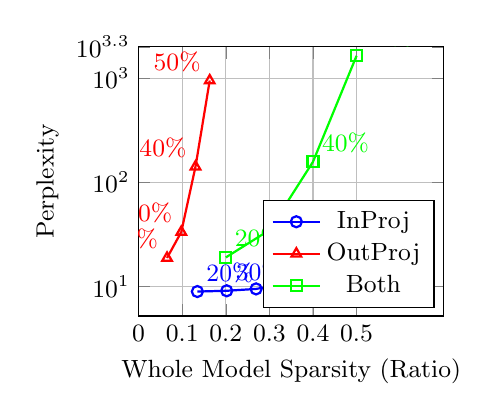
\begin{tikzpicture}
\small
    \begin{axis}[
        width=.45\textwidth, height=5cm,
        xlabel={Whole Model Sparsity (Ratio)},
        ylabel={Perplexity},
        legend pos=south east,
        grid=both,
        xmin=0.0, xmax=0.7,
        ymin=0., ymax=2000,
        ymode=log,
        log basis y=10,
        xtick={0, 0.1,  0.2,  0.3,  0.4, 0.5},
        ytick={1, 10, 100, 1000, 2000},
    ]
        % In_Proj data
        \addplot[
            color=blue,
            mark=o,
            thick
        ] coordinates {
            (0.3369, 10.5762)
            (0.2695, 9.4666)
            (0.2021, 9.0830)
            (0.1348, 8.9316)
        };
        \addlegendentry{\small \inproj}

        % Adding pruning ratio labels for In_Proj
        \node at (axis cs:0.3369,10.5762) [anchor=south west, blue] {50\%};
        \node at (axis cs:0.2695,9.4666) [anchor=south west, blue] {40\%};
        \node at (axis cs:0.2021,9.0830) [anchor=south west, blue] {30\%};
        \node at (axis cs:0.1348,8.9316) [anchor=south west, blue] {20\%};

        % Out_Proj data
        \addplot[
            color=red,
            mark=triangle,
            thick
        ] coordinates {
            (0.1631, 948.7922)
            (0.1305, 141.4194)
            (0.0979, 33.3519)
            (0.0652, 18.7741)
        };
        \addlegendentry{\small \outproj}

        % Adding pruning ratio labels for Out_Proj
        \node at (axis cs:0.1631,948.7922) [anchor=south east, red] {50\%};
        \node at (axis cs:0.1305,141.4194) [anchor=south east, red] {40\%};
        \node at (axis cs:0.0979,33.3519) [anchor=south east, red] {30\%};
        \node at (axis cs:0.0652,18.7741) [anchor=south east, red] {20\%};

        % All (New Data Group)
        \addplot[
            color=green,
            mark=square,
            thick
        ] coordinates {
            (0.5000, 1639.3659)
            (0.4000, 157.2813)
            (0.3000, 34.7289)
            (0.2000, 18.9848)
        };
        \addlegendentry{\small Both}

        % Adding pruning ratio labels for All
        \node at (axis cs:0.5000,1639.3659) [anchor=south west, green] {50\%};
        \node at (axis cs:0.4000,157.2813) [anchor=south west, green] {40\%};
        \node at (axis cs:0.3000,34.7289) [anchor=south west, green] {30\%};
        \node at (axis cs:0.2000,18.9848) [anchor=south west, green] {20\%};

    \end{axis}
\end{tikzpicture}

\caption{The effect of different unstructured (WANDA) pruning ratios on different components of \textsc{\mambab-2.7B}~(\inproj, \outproj, and full model pruning). The numbers represent the pruning ratio of the specific layer. We observe that the out-projection layer is substantially more sensitive to pruning than the in-projection layer.}
\label{fig:perplexity_plot}
\end{figure}

%\newpage

\section*{Limitations}
Drawing direct conclusions from our experiments is not straightforward. The four LLMs we experiment with differ, among other, in size, head pattern, training data, and structure. These choices are due to the scarcity of SSM-based LLMs, and the computational costs of training or distilling various models to control for specific variables.

In addition, the structure pruning methods we consider also differ in their effect on the models, as indicated by the different compression ratios in \cref{tab:ratio_pruning,tab:heads_pruning}. The challenges here stem from the different constraints imposed by the different methods. E.g., in state pruning we prune $BC$-heads, which cap the compression by the number of parameters \wb~and \wc~occupy in the \mambab component, especially when the model configuration is GVA which translates to fewer $BC$-heads. Another example is when pruning Head-Dim we are obliged to prune large portions of \outproj to keep dimensionality correctness in the flow, leading to pruning potentially important parameters from it.

Despite these issues, we believe the signals we observe are valuable. For instance, the robustness of SSM-based LLMs to state pruning is demonstrated by the modest performance drop for 50\% pruning ratios~(e.g., a 1\% drop both with a 20\% compression ratio for in \textsc{\phimamba}, and 25\% compression ratio for \textsc{\smol}), compared to a huge drop with head pruning for a 25\% pruning ratio, sometimes with the same model~(e.g., a 30\% drop for both \textsc{\hybridmamba} and \textsc{\smol} with 5\% compression ratio). 



We also focused our experiments exclusively on pruning the \mambab components and excluded feed-forward networks, assuming that prior work on transformer pruning had already addressed those extensively. Future work will address pruning the all model components to study the interaction between the different components, as well as potential to get more significant computational savings. 

\section*{Acknowledgments}
We thank Jana Omary Ghattas for her help in creating \cref{fig:mamba2arch}. We also thank Yuval Reif for his support. 
This work was supported in part by the Israel Science Foundation (grant no. 2045/21).



\bibliography{custom, anthology}

\newpage

\appendix
\section{Selecting the Loss Function}
Recovering performance in purned models is usually done by finetuning the model on a calibration dataset, however, this comes with the risk of over-fitting the dataset or regaining performance back in the area the dataset focuses on. Therefore, we checked the effect of using KD loss instead of Cross-Entropy~(CE) loss in the data set. As can be seen in~\cref{tab:CEvsKD}, it is clear that using KD loss helps the model regain overall performance along most benchmarks, while using CE, the model regains some performance in some tasks~(e.g., lambada) but doesn't improve much on other benchmarks.
\label{sec:appendix}
\begin{table*}
\centering
\small
\begin{tabular}{lccccccc}
\hline
{} &  arc\_challenge &  arc\_easy &  hellaswag &  lambada\_openai &   piqa &  winogrande &  Average \\
\hline
Baseline &         0.418 &    0.739 &     0.461 &          0.500 & 0.755 &      0.716 &   0.598 \\
w/o FT. &         0.378 &    0.713 &     0.433 &          0.349 & 0.747 &      0.651 &   0.545 \\
CE loss &         0.385 &    0.721 &     0.413 &          0.405 & 0.748 &      0.682 &   0.559 \\
KD loss &         0.410 &    0.726 &     0.454 &          0.452 & 0.753 &      0.693 &   0.581 \\
\hline
\end{tabular}
\caption{\label{tab:CEvsKD}
    Comparing loss choice. \phimamba with pruned SSM states according to Taylor importance estimation,  by 50\% 
 and fine-tuning using LoRA with different losses. The baseline model is the (full) fine-tuned model. KD loss consistently outperforms CE loss.
  }
\end{table*}


\section{Experimental Details}\label{app:exp_setup}
We finetune all models for 10K steps with batch size of 6 and learning rate of $5e-5$, using bf16. We use LoRA with rank=8 and $\alpha$=16.
We run our experiments on a single NVIDIA A100 80GB.



\section{Full Results}
\label{app:all_results}
\Cref{tab:headdim_full,tab:wanda_full,tab:merge_full,tab:baselines_full,tab:flap_results,tab:state_results} show our results on all benchmarks for the different models.

\begin{table}[ht]
\centering
\small
\begin{tabular}{lccccccccc}
\toprule
Model & Ratio & FT & arc\_challenge & arc\_easy & hellaswag & lambada & piqa & winogrande  \\
\midrule
\hybridmamba & 0.25 & w/o & 0.18 & 0.37 & 0.27 & 0.06 & 0.54 & 0.51  \\
\hybridmamba & 0.25 & w/  & 0.20 & 0.34 & 0.27 & 0.06 & 0.56 & 0.51  \\
\hybridmamba & 0.50 & w/o & 0.22 & 0.26 & 0.26 & 0.00 & 0.55 & 0.50  \\
\hybridmamba & 0.50 & w/  & 0.17 & 0.35 & 0.27 & 0.06 & 0.56 & 0.51  \\
\phimamba   & 0.50 & w/o & 0.18 & 0.40 & 0.27 & 0.00 & 0.60 & 0.52   \\
\phimamba   & 0.50 & w/  & 0.29 & 0.65 & 0.38 & 0.22 & 0.71 & 0.54   \\
\phimamba   & 0.25 & w/o & 0.25 & 0.60 & 0.30 & 0.06 & 0.69 & 0.50   \\
\phimamba   & 0.25 & w/  & 0.36 & 0.70 & 0.42 & 0.35 & 0.74 & 0.63   \\
\mambab-2.7B & 0.25 & w/o & 0.21 & 0.27 & 0.26 & 0.00 & 0.53 & 0.50  \\
\mambab-2.7B & 0.25 & w/  & 0.22 & 0.25 & 0.26 & 0.00 & 0.52 & 0.45  \\
\mambab-2.7B & 0.50 & w/o & 0.22 & 0.26 & 0.25 & 0.00 & 0.52 & 0.50  \\
\mambab-2.7B & 0.50 & w/  & 0.23 & 0.26 & 0.26 & 0.00 & 0.53 & 0.50  \\
\smol       & 0.25 & w/o & 0.22 & 0.25 & 0.26 & 0.00 & 0.52 & 0.49   \\
\smol       & 0.25 & w/  & 0.18 & 0.33 & 0.26 & 0.00 & 0.55 & 0.52   \\
\smol       & 0.50 & w/o & 0.20 & 0.26 & 0.26 & 0.00 & 0.50 & 0.49   \\
\smol       & 0.50 & w/  & 0.19 & 0.32 & 0.26 & 0.00 & 0.54 & 0.51   \\
\bottomrule
\end{tabular}
\caption{Head dimension pruning benchmarks results.}
\label{tab:headdim_full}
\end{table}

\begin{table}[ht]
\centering
\small
\begin{tabular}{l c c c c c c c}
\toprule
Model         & Ratio & arc\_challenge & arc\_easy & hellaswag & lambada & piqa & winogrande \\
\midrule
\phimamba     & 0.25  & 0.41           & 0.74      & 0.46      & 0.50    & 0.76 & 0.72 \\
\phimamba     & 0.50  & 0.39           & 0.72      & 0.45      & 0.40    & 0.75 & 0.69 \\
\mambab-2.7B  & 0.25  & 0.31           & 0.63      & 0.42      & 0.49    & 0.72 & 0.58 \\
\mambab-2.7B  & 0.50  & 0.20           & 0.35      & 0.28      & 0.02    & 0.57 & 0.54 \\
\hybridmamba  & 0.25  & 0.51           & 0.80      & 0.55      & 0.55    & 0.77 & 0.68 \\
\hybridmamba  & 0.50  & 0.51           & 0.80      & 0.54      & 0.54    & 0.76 & 0.66 \\
\smol         & 0.25  & 0.42           & 0.75      & 0.50      & 0.56    & 0.77 & 0.63 \\
\smol         & 0.50  & 0.37           & 0.72      & 0.47      & 0.42    & 0.76 & 0.59 \\
\bottomrule
\end{tabular}
\caption{WANDA pruning benchmarks results.}
\label{tab:wanda_full}
\end{table}

\clearpage
\begin{table}[ht]
\centering
\small
\begin{tabular}{l c c c c c c c c}
\toprule
model    & Heads & FT & arc\_challenge & arc\_easy & hellaswag & lambada & piqa & winogrande \\
\midrule
\phimamba         & 16  & w/o & 0.39 & 0.72 & 0.47 & 0.42 & 0.75 & 0.59 \\
\phimamba         & 16  & w/  & 0.45 & 0.73 & 0.49 & 0.43 & 0.76 & 0.62 \\
\phimamba         & 8   & w/o & 0.38 & 0.71 & 0.46 & 0.41 & 0.74 & 0.57 \\
\phimamba         & 8   & w/  & 0.41 & 0.72 & 0.47 & 0.42 & 0.75 & 0.58 \\
\mambab-2.7B      & 40  & w/o & 0.21 & 0.27 & 0.26 & 0.00 & 0.52 & 0.50 \\
\mambab-2.7B      & 40  & w/  & 0.21 & 0.27 & 0.25 & 0.00 & 0.52 & 0.50 \\
\mambab-2.7B      & 20  & w/o & 0.21 & 0.26 & 0.26 & 0.00 & 0.51 & 0.48 \\
\mambab-2.7B      & 20  & w/  & 0.21 & 0.26 & 0.26 & 0.00 & 0.52 & 0.48 \\
\smol             & 16  & w/o & 0.20 & 0.27 & 0.26 & 0.00 & 0.53 & 0.49 \\
\smol             & 16  & w/  & 0.27 & 0.59 & 0.41 & 0.14 & 0.70 & 0.53 \\
\smol             & 8   & w/o & 0.22 & 0.26 & 0.26 & 0.00 & 0.52 & 0.48 \\
\smol             & 8   & w/  & 0.32 & 0.66 & 0.40 & 0.25 & 0.72 & 0.54 \\
\hybridmamba      & 4   & w/o & 0.20 & 0.25 & 0.24 & 0.00 & 0.50 & 0.47 \\
\hybridmamba      & 4   & w/  & 0.22 & 0.27 & 0.26 & 0.00 & 0.53 & 0.50 \\
\hybridmamba      & 2   & w/o & 0.21 & 0.24 & 0.25 & 0.00 & 0.51 & 0.46 \\
\hybridmamba      & 2   & w/  & 0.23 & 0.28 & 0.27 & 0.00 & 0.54 & 0.49 \\
\bottomrule
\end{tabular}
\caption{Head merging benchmarks results.}
\label{tab:merge_full}
\end{table}
       
\begin{table}[ht]
\centering
\small
\begin{tabular}{lccccccc}
\toprule
model   & arc\_challenge & arc\_easy & hellaswag & lambada & piqa & winogrande \\
\midrule
\smol              & 0.43 & 0.75 & 0.51 & 0.57 & 0.77 & 0.63 \\
\mambab-2.7B       & 0.33 & 0.70 & 0.50 & 0.70 & 0.76 & 0.64 \\
\phimamba          & 0.41 & 0.74 & 0.46 & 0.50 & 0.76 & 0.72 \\
\hybridmamba       & 0.51 & 0.80 & 0.55 & 0.55 & 0.77 & 0.67 \\
\bottomrule
\end{tabular}
\caption{Models baseline results for the benchmarks.}
\label{tab:baselines_full}
\end{table}

\clearpage
\begin{table}[ht]
\centering
\small
\begin{tabular}{l c c c c c c c}
\toprule
\textbf{Model}    & \textbf{Ratio} & \textbf{arc\_challenge} & \textbf{arc\_easy} & \textbf{hellaswag} & \textbf{lambada} & \textbf{piqa} & \textbf{winogrande} \\
\midrule
\phimamba         & 0.25 & 0.39 & 0.72 & 0.44 & 0.44 & 0.75 & 0.66 \\
\phimamba         & 0.50 & 0.34 & 0.69 & 0.40 & 0.17 & 0.74 & 0.58 \\
\hybridmamba      & 0.25 & 0.22 & 0.27 & 0.26 & 0.00 & 0.52 & 0.49 \\
\hybridmamba      & 0.50 & 0.24 & 0.27 & 0.26 & 0.00 & 0.51 & 0.45 \\
\mambab-2.7B      & 0.25 & 0.23 & 0.28 & 0.25 & 0.00 & 0.51 & 0.48 \\
\mambab-2.7B      & 0.50 & 0.25 & 0.28 & 0.25 & 0.02 & 0.50 & 0.44 \\
\smol             & 0.25 & 0.34 & 0.69 & 0.44 & 0.27 & 0.74 & 0.55 \\
\smol             & 0.50 & 0.26 & 0.57 & 0.37 & 0.06 & 0.69 & 0.52 \\
\bottomrule
\end{tabular}
\caption{FLAP benchmarks results.}
\label{tab:flap_results}
\end{table}


\begin{table}[ht]
\centering
\small
\begin{tabular}{l c c c c c c c c}
\toprule
\textbf{Model}    & \textbf{Ratio} & \textbf{FT} & \textbf{arc\_challenge} & \textbf{arc\_easy} & \textbf{hellaswag} & \textbf{lambada} & \textbf{piqa} & \textbf{winogrande} \\
\midrule
\hybridmamba  & 0.25 & w/o & 0.25 & 0.25 & 0.24 & 0.02 & 0.49 & 0.49 \\
\hybridmamba  & 0.25 & w/  & 0.26 & 0.27 & 0.25 & 0.01 & 0.51 & 0.50 \\
\hybridmamba  & 0.50 & w/o & 0.23 & 0.24 & 0.26 & 0.02 & 0.50 & 0.49 \\
\hybridmamba  & 0.50 & w/  & 0.17 & 0.35 & 0.27 & 0.06 & 0.56 & 0.51 \\
\mambab-2.7B  & 0.25 & w/o & 0.30 & 0.59 & 0.37 & 0.32 & 0.7 & 0.59 \\
\mambab-2.7B  & 0.25 & w/  & 0.31 & 0.59 & 0.38 & 0.32 & 0.69 & 0.59 \\
\mambab-2.7B  & 0.50 & w/o & 0.30 & 0.57 & 0.37 & 0.32 & 0.69 & 0.59 \\
\mambab-2.7B  & 0.50 & w/  & 0.30 & 0.57 & 0.38 & 0.32 & 0.69 & 0.59 \\
\phimamba & 0.25 & w/o & 0.40 & 0.73 & 0.45 & 0.36 & 0.75 & 0.67 \\
\phimamba & 0.25 & w/  & 0.40 & 0.74 & 0.46 & 0.46 & 0.75 & 0.71 \\
\phimamba & 0.50 & w/o & 0.38 & 0.71 & 0.43 & 0.34 & 0.75 & 0.65 \\
\phimamba & 0.50 & w/  & 0.41 & 0.72 & 0.45 & 0.45 & 0.75 & 0.69 \\
\smol         & 0.25 & w/o & 0.40 & 0.73 & 0.48 & 0.53 & 0.76 & 0.61 \\
\smol         & 0.25 & w/  & 0.42 & 0.74 & 0.50 & 0.55 & 0.77 & 0.62 \\
\smol         & 0.50 & w/o & 0.31 & 0.63 & 0.40 & 0.27 & 0.70 & 0.52 \\
\smol         & 0.50 & w/  & 0.40 & 0.74 & 0.49 & 0.54 & 0.76 & 0.60 \\
\bottomrule
\end{tabular}
\caption{\label{tab:state_results} State pruning benchmarks full results.}
\end{table}


\end{document}
